\documentclass[border=2pt]{standalone}
\usepackage[T1]{fontenc}
\usepackage{mathptmx}
\usepackage{tikz}
\usetikzlibrary{arrows.meta,positioning,fit,calc,shapes.geometric,backgrounds}
\usepackage{siunitx}
\tikzset{
  >={Stealth[length=1.8mm]},
  blk/.style={draw, thick, minimum height=11mm, text width=16mm, align=center, font=\scriptsize, inner sep=1.5pt, fill=white},
  lab/.style={font=\scriptsize, align=center},
  every picture/.style={line width=0.6pt},
}

% One-column state diagram of rtl/cmd_ctrl.v (about 80 mm wide, drawn at print size).
\begin{document}
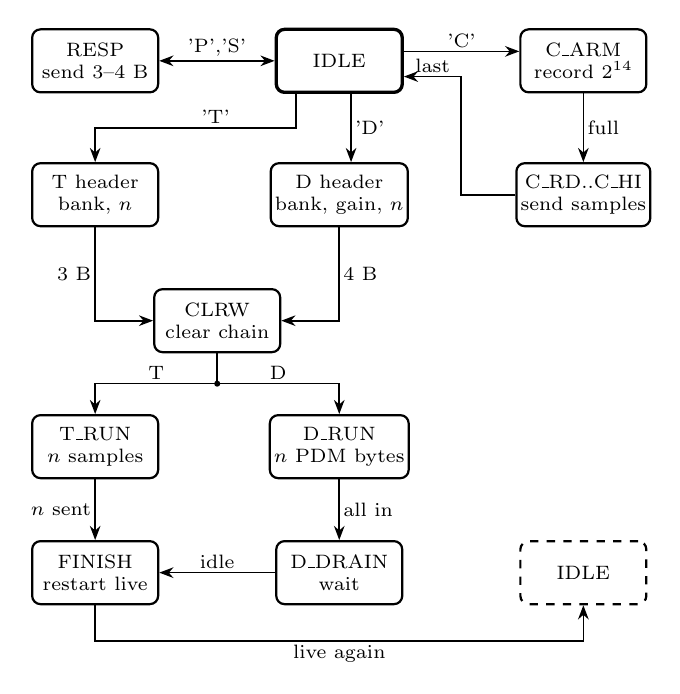
\begin{tikzpicture}[s/.style={draw, thick, rounded corners=3pt, minimum height=8mm, minimum width=16mm, font=\scriptsize, align=center, fill=white, inner sep=1.5pt},
  el/.style={font=\scriptsize, align=center, inner sep=1.2pt}]
\node[s] (resp)  at (0.9, 0)    {RESP\\send 3--4 B};
\node[s, line width=1.2pt] (idle) at (4.0, 0) {IDLE};
\node[s] (carm)  at (7.1, 0)    {C\_ARM\\record $2^{14}$};
\node[s] (th)    at (0.9,-1.7)  {T header\\bank, $n$};
\node[s] (dh)    at (4.0,-1.7)  {D header\\bank, gain, $n$};
\node[s] (cd)    at (7.1,-1.7)  {C\_RD..C\_HI\\send samples};
\node[s] (clrw)  at (2.45,-3.3) {CLRW\\clear chain};
\node[s] (trun)  at (0.9,-4.9)  {T\_RUN\\$n$ samples};
\node[s] (drun)  at (4.0,-4.9)  {D\_RUN\\$n$ PDM bytes};
\node[s] (fin)   at (0.9,-6.5)  {FINISH\\restart live};
\node[s] (dd)    at (4.0,-6.5)  {D\_DRAIN\\wait};
\node[s, dashed] (idle2) at (7.1,-6.5) {IDLE};
\draw[<->] (resp) -- node[el, above]{'P','S'} (idle);
\draw[->] ($(idle.east)+(0,0.12)$) -- node[el, above]{'C'} ($(carm.west)+(0,0.12)$);
\draw[->] (carm) -- node[el, right]{full} (cd);
\draw[->] (cd.west) -- (5.55,-1.7) |- node[el, above, pos=0.75]{last} ($(idle.east)+(0,-0.2)$);
\draw[->] ($(idle.south)+(-0.55,0)$) |- node[el, above, pos=0.7]{'T'} (0.9,-0.85) -- (th.north);
\draw[->] (idle.south -| 4.15,0) -- node[el, right]{'D'} (dh.north -| 4.15,0);
\draw[->] (th) |- node[el, pos=0.25, left]{3 B} (clrw.west);
\draw[->] (dh) |- node[el, pos=0.25, right]{4 B} (clrw.east);
\draw (clrw.south) -- (2.45,-4.1);
\draw[->] (2.45,-4.1) -| node[el, above, pos=0.25]{T} (trun.north);
\draw[->] (2.45,-4.1) -| node[el, above, pos=0.25]{D} (drun.north);
\fill (2.45,-4.1) circle (1.1pt);
\draw[->] (trun) -- node[el, left]{$n$ sent} (fin);
\draw[->] (drun) -- node[el, right]{all in} (dd);
\draw[->] (dd) -- node[el, above]{idle} (fin);
\draw[->] (fin.south) -- ++(0,-0.45) -| node[el, pos=0.25, below]{live again} (idle2.south);
\end{tikzpicture}
\end{document}
